\section{Results}
\subsection{Time-to-correct solution}
Cumulatively, across the four tasks, we did not observe a significant change
in the time-to-correct solution.
%
A Wilcoxon Rank-Sum test, performed on the aggregate of per-task rankings,
yielded a confidence interval $p=0.14$.
%
Performing rank-sum of ranks is an especially conservative test, because it weighs
per-task rankings equally, regardless of the absolute times.

Although the results do not indicate a change across the board, our data shows a dramatic
speedup for the example group in Task 2 (see Figure~\ref{fig:data-points}).
%
This may indicate that certain tasks benefit from examples while others do not.
%
We discuss this more thoroughly in Section~\ref{sec:discussion}

\subsection{Incorrect guesses}
\subsection{Interpreter usage}
% Figures.
\begin{figure*}[ht]
  \centering
  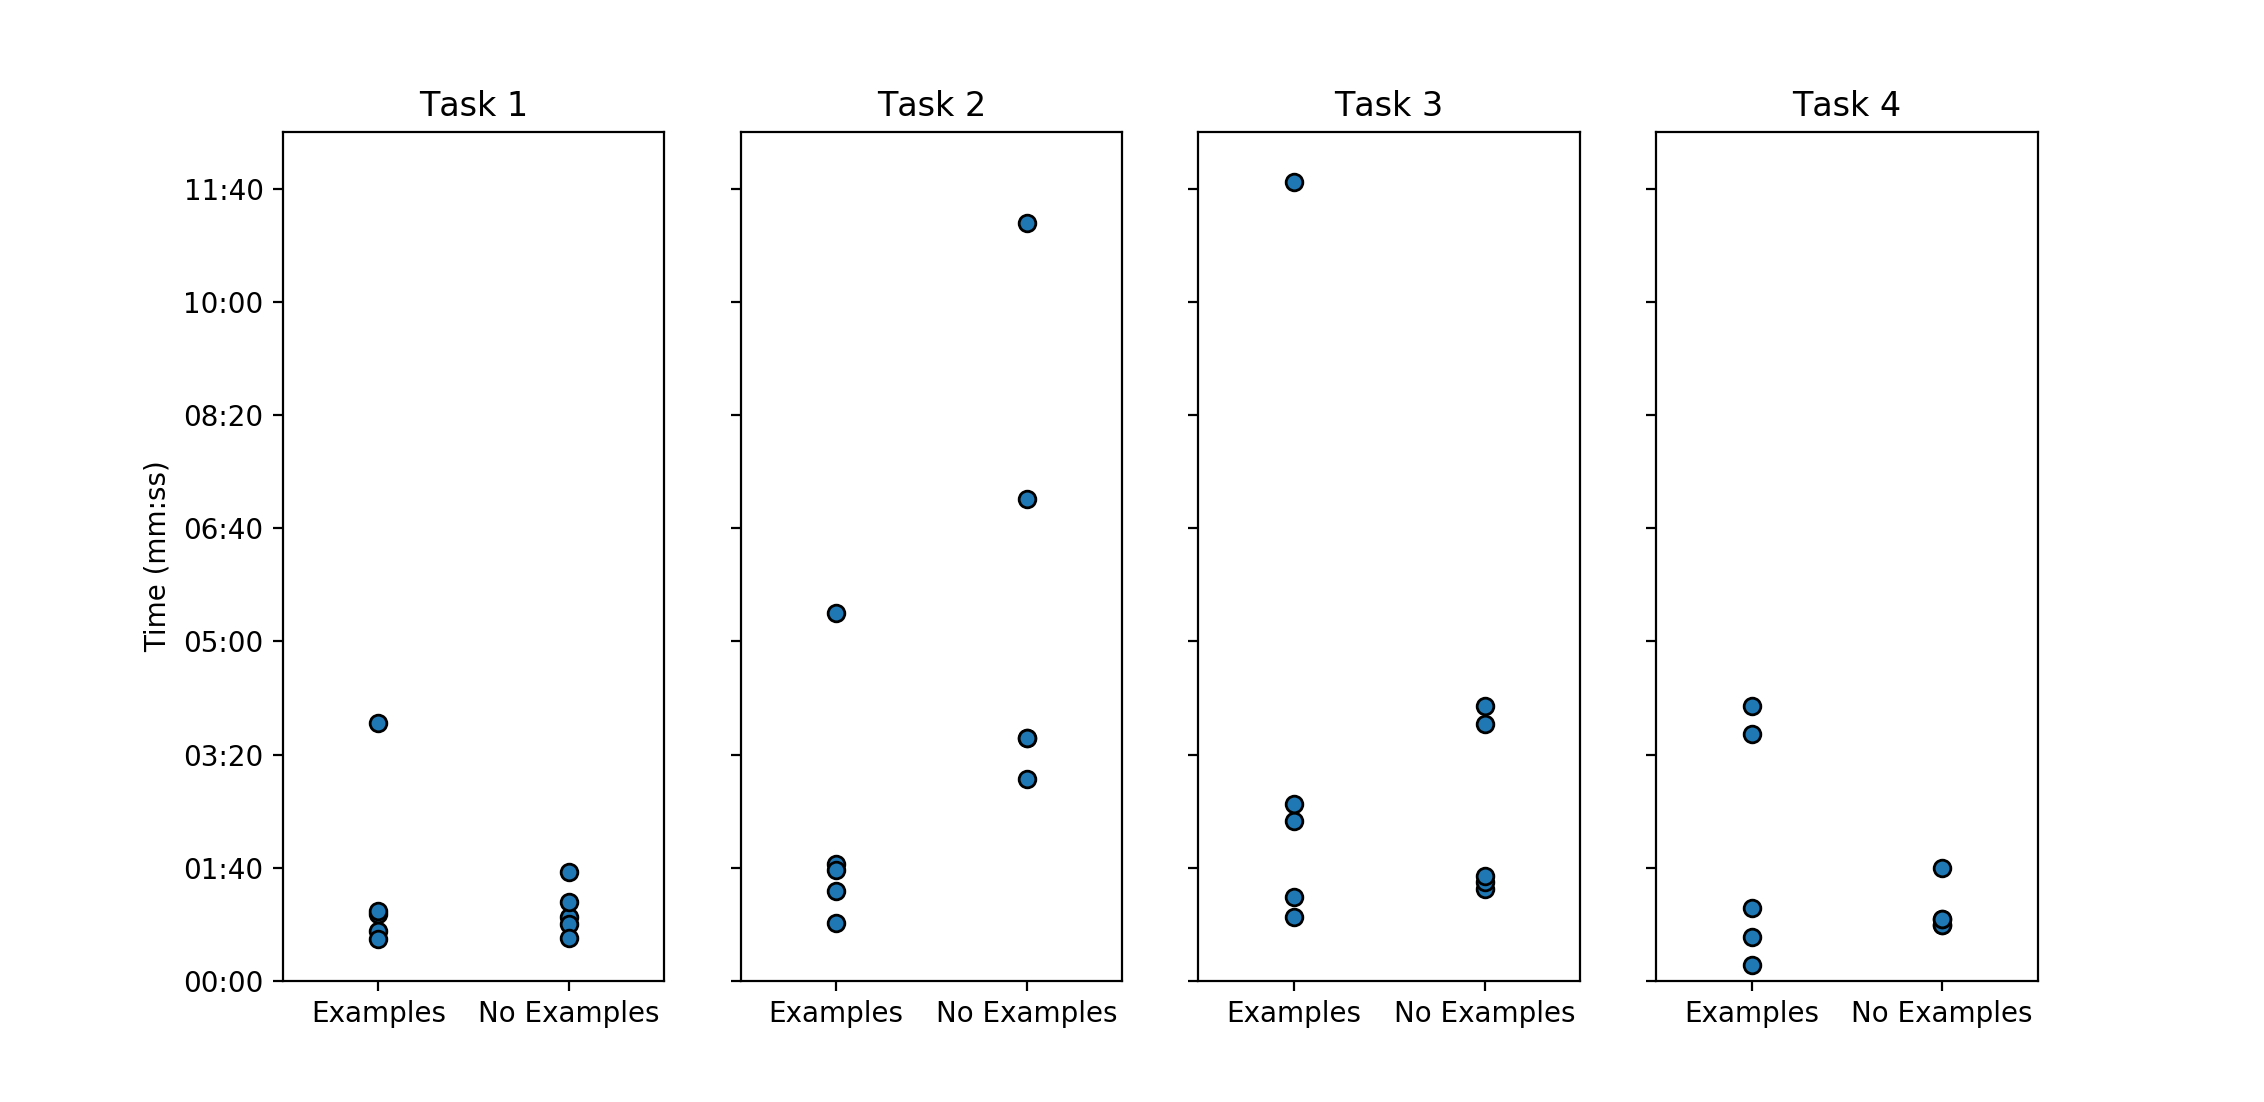
\includegraphics[width=\textwidth]{results/task_points.png}
  \caption{
    Examples did not noticeably affect time-to-completion, except in Task 2
    where the effect is dramatic.
  }
  \label{fig:data-points}
\end{figure*}